%----------------------------------------------------------------------------
\chapter{Test Implementation and Execution for MoDeS$^3$ project}\label{TestImpl:MODES}
%----------------------------------------------------------------------------

\section{Test Environment Readiness Report}
\paragraph{Hardware} The entire table have been properly set up in a university laboratory.
\paragraph{Software} The Eclipse Photon (4.8.0) have been set up with the necessary dependencies (Gradle, Java, Viatra, Xtend, Xtext, E(fx)clipse) and for deployment purposes a linux-subsystem for windows have been accepted.

\section{Test Implementation}
This section describes the technical details of test implementation and execution for each test plans of MoDeS$^3$ project.
\paragraph{Deploying} For implementation and testing purposes it is not recommended to use the real microcontrollers (BBB, Pi or Arduino itself). During my thesis work, I have used Windows 10 operating system with Eclipse and Visual Studio Code (which are available also for Unix and Mac systems), but for deploying purposes the MoDeS$^3$ team uses Ansible\footnote{For more info visit \url{https://www.ansible.com/} site.}, which is not available for Windows systems. Fortunately there is an option to create unix subsystem inside a Windows operating system, where from I have managed to deploy the necessary components to the BBB.

\subsection{Unit tests} Considering the unit test feature sets (\autoref{table:Feature-Sets-Unit}), the GPIO Manager, Occupancy Query, Track Element Controller, Safety Logic and Dashboard components are written in Java or Xtend\footnote{Xtend is a general purpose programming language, from which java code is generate. More information is available here: \url{https://www.eclipse.org/xtend/documentation/index.html}} languages and the Section Occupancy Query is implemented in C++ for the Arduino. 

The first task is to set up the proper environment in Eclipse with Gradle and JUnit 5 \cite{JUnit5} plugins to test Java components. To create additional objects for verification and faking purposes (like avoid using file operations during testing), Mockito \cite{Mockito} and PowerMock \cite{PowerMock} was added to the environment. The first extension is inheriting the objects, which should be faked in the test and replacing it in the background to a fake object. These objects will behave as the test case requires them, like returning a specific value for the exact parameters. Additionally these objects can also be verified that how many times and with which parameters they have been called. The PowerMock extends these functionalities with faking for example static and private methods, which can not be done with an inheritance (so with Mockito framework). Unfortunately the JUnit team have not yet implemented the possibility to use PowerMock in JUnit 5 tests, but the framework supports running JUnit 4 tests. To summarize that, with the setup of JUnit 5 and PowerMock for Mockito we can test static methods (which is commonly used for Singleton pattern). Each component must reach an 80\% of code coverage defined by the Unit Test Plan. Although the measurement could not be run with jacoco plugin, because it does not applicable for Xtend programming language. One alternative tool is the EclEmma\footnote{The plugin and their usage is described here: \url{https://www.eclemma.org/}} Eclipse plugin.

For the C++ language based Section Occupancy Query component it is advised to use Visual Studio Code with PlatformIO extension\footnote{Detailes about the framework are available here: \url{https://platformio.org/}}. The tests can be implemented for this component in the Google Test framework\footnote{Introduction can be found here:\url{https://github.com/google/googletest}}.

\paragraph{FS-1: GPIO Handling} The handling of GPIO pins is based on the GPIO sysfs interface\footnote{Interface is explained here in details: \url{https://www.kernel.org/doc/Documentation/gpio/sysfs.txt}}, which provides a file based GPIO controlling with \textit{/sys/class/gpio/} root folder for unix systems. Therefore the GPIO Manager Java component must handle file operations in the specific folders. In order to test the logic regarding GPIO handling, the file writing and reading operations must be extracted into separate classes.

\begin{figure}[ht]
	\centering
	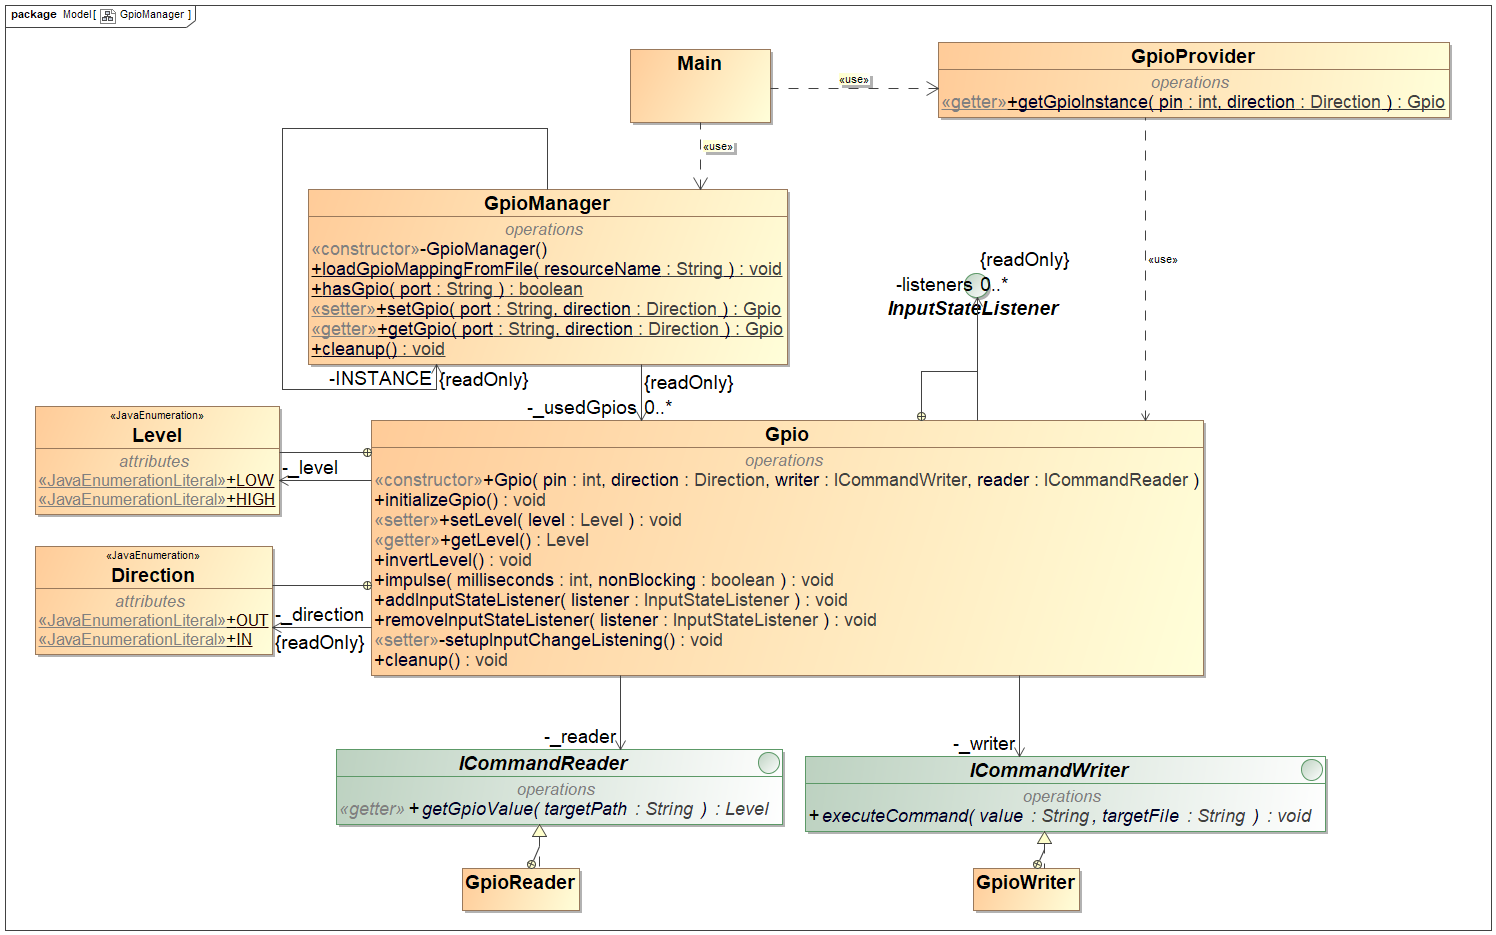
\includegraphics[width=150mm, keepaspectratio]{figures/impl/GpioManager.png}
	\caption{Gpio manager class diagram}
	\label{fig:gpiomanagerClass}
\end{figure}
On \autoref{fig:gpiomanagerClass}, a class diagram shows the re-factored structure of the component. This structure gives an advantage that the file operation dependencies are extracted into interfaces, which we can be easily mocked. The following code snippet shows how a fake object can be created and verified. 

\begin{lstlisting}[language = Java]
private static final String GPIOFOLDER = "/sys/class/gpio/";
// Create a fake class which behaves as any ICommandWriter class
@Mock
private ICommandWriter writer = Mockito.mock(ICommandWriter.class);
// Verify that the 'writer' fake object have been called 
// with 1 time during the execution with these exact parameters
Mockito.verify(writer, Mockito.times(1)).executeCommand(String.valueOf(67), GPIOFOLDER + "export");
\end{lstlisting}

As explained before the static methods can only be mocked with PowerMock, thus the following example shows how to make the GpioProvider to return a fake Gpio instance when the \textit{getGpioInstance} method is called with parameters: 86, Gpio.Direction.IN. Therefore in any further tests we can examine the mGpio instance as explained before.

\begin{lstlisting}
@RunWith(PowerMockRunner.class)
@PrepareForTest(GpioProvider.class)
public class GpioManagerTest{
	@Mock
	private Gpio mGpio = Mockito.mock(Gpio.class);
	
	@Before
	public void initEnv(){
		// Setup powermockito for static GpioProvider mocking
		PowerMockito.mockStatic(GpioProvider.class);
		// For these specific parameters, return the mGpio parameter
		PowerMockito.when(GpioProvider.getGpioInstance(86, Gpio.Direction.IN)).thenReturn(mGpio);
	}
}
\end{lstlisting}

Naturally a unit test should cover only one class, consequently if we consider the previously described structure (shown in \autoref{fig:gpiomanagerClass}), 6 unit test classes should be created (note that Level and Direction objects are only enumerables). Although there is no need to test basic file operation functions, provided by the Java framework in the GpioWriter and GpioReader classes and in addition there is no advantage to test the Main and GpioProvider classes, because there is complex logic which should be verified by a test.


\paragraph{FS-2: Occupancy detection} The occupancy information handling components are the Section Occupancy Query (in C++ language) and the Occupancy Query elements (written in Xtend). The information flow between these components is based on S88 serial port connection. In this case this test implementation requires an S88 connection to the Arduino hardware element, because there is no virtual serial port simulators for Windows available on the market. Otherwise the C++ component can be separately verified that, it is collecting all the informations from the sections with Google Test. The Occupancy Query component runs on Java Virtual Machine, so JUnit 5 can be used without a problem. 

\begin{figure}[ht]
	\centering
	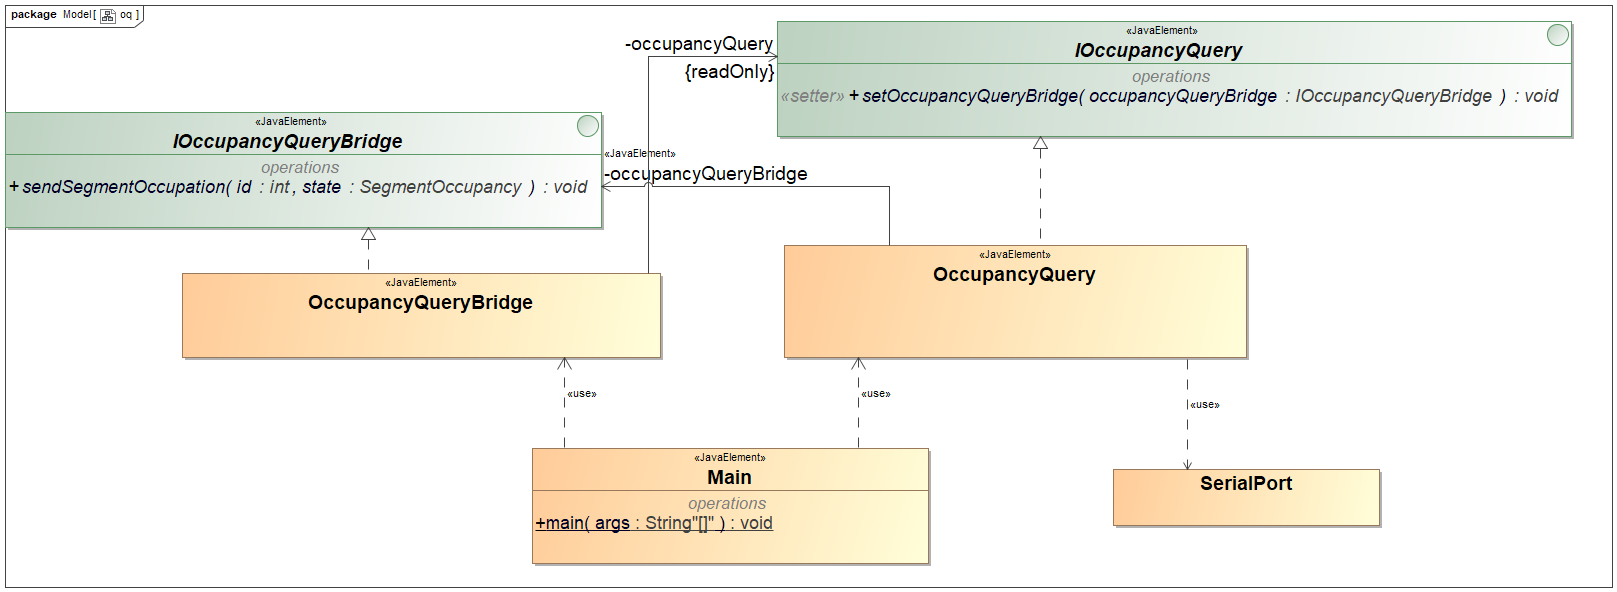
\includegraphics[width=150mm, keepaspectratio]{figures/impl/oq.png}
	\caption{Occupancy Query class diagram}
	\label{fig:occupancyqueryClass}
\end{figure}
The class structure of the Occupancy Query component is shown in \autoref{fig:occupancyqueryClass}, which describes the separation of a OccupancyQueryBridge, OccupancyQuery and Main class with their interfaces. The advantage of this architecture is the Occupancy calculation logic is well-separated from the message handling (in the OccupancyQueryBridge) logic. The obstacle to implement hardware independent test cases is the serial port dependency in the OccupancyQuery, for which the component must be re-factored. In addition the OccupancyQuery have dependencies to the SegmentOccupancy message type and for message handling elements, which should be also faked during the test executions.

\paragraph{FS-3: Track element controller} The next component have additional dependencies to the Turnout and SegmentState messages, to be able to perceive any state change on the track. In order to supervise the sections, the Track element controller must rely on the messaging service component aligned with the track configuration properties. The currently applicable version from the PowerMock is still in beta state, but until this point it was working properly. Unfortunately I have faced an issue, when I tried to mock a static method with a parameter of a static instance. The PowerMock already assigned the issue, but there is no bugfix implementation yet for the problem. Apart from that the architecture can also be reviewed to avoid static classes where it is not necessary.

\paragraph{FS-4: Safety Logic} The component level implementation of the Safety Logic is consist of high level model based validators, from which a Java code was generated. In addition there is no need to test the glue code for these generated models. The system level Safety Logic also relies on generated Java code from the EMF model, nevertheless the decision-making logic is written in Xtend. This implementation also follows the previously described application and communication bridge architecture, but have a purely separated track refreshing algorithm. There are several shutdown strategies, which can be tested with this algorithm together. In addition this component also have dependencies to the SendAllStatus, SegmentOccupancy, TurnoutState, SegmentState and ComputerVisionObjectPositions messages with the communication services also.

\paragraph{FS-5: DashBoard} This feature set and component is responsible for controlling and visualizing the status of the track elements. Therefore it is handling mainly message communication and there was no need to implement test cases for this component.
\todo[inline]{there was no need to test this}

\subsection{Integration tests}
There is separate component for the integration test purposes, which shows an example how to initialize and send messages to communication topics through the network. This component was not further extended for the integration test cases.

\subsection{System tests}
In order to execute system tests the demonstrator table must be started properly with the safety logic also. To start when the table is switched on, the BBB, PI and Arduino hardware elements are configured to start automatically with the basic services. These are the SectionOccupancyQuery, OccupancyQuery, TrackElementController and Dashboard components. The Safety Logic implementations prerequisites are to have these services already running on the network. Therefore after every automatically starting service is up, the component level safety logic service can be started on every BBB.\footnote{More information about starting the demonstrator system can be found here: \url{https://github.com/FTSRG/BME-MODES3/wiki/Starting-the-demonstrator}}

\section{Test Results}
\begin{figure}[ht]
	\centering
	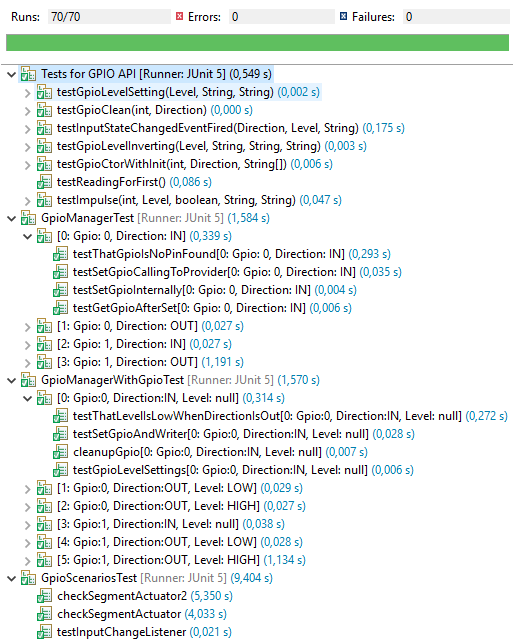
\includegraphics[width=100mm, keepaspectratio]{figures/impl/gpioTests.png}
	\caption{Implemented test cases for GPIO Manager component}
	\label{fig:gpiomanagerTests}
\end{figure}
Thus I have implemented unit test classes for Gpio and GpioManager separately (shown as "Tests for GPIO API" and "GpioManagerTest" groups on \autoref{fig:gpiomanagerTests}), then test cases for verifying the GpioManager with Gpio together. The GpioScenariosTest is stands for running an initialization test with all the components together in the final environment (in Debian operating system on the BBB). All the previous test classes are parameterized with more than one GPIO pin and all (in and out) directions.

\begin{figure}[ht]
	\centering
	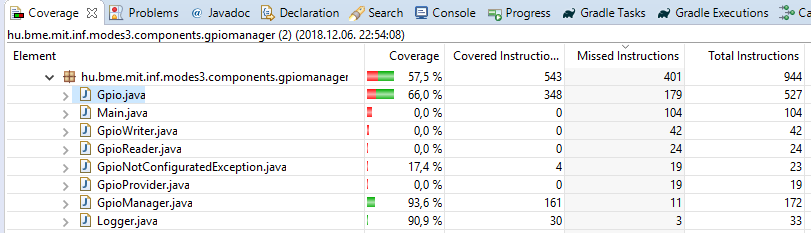
\includegraphics[width=150mm, keepaspectratio]{figures/impl/gpioCoverage.png}
	\caption{Code coverage measurement for GPIO Manager component}
	\label{fig:gpiomanagerCoverage}
\end{figure}
For each component the requirement was to achieve an 80\% code coverage. It is unnecessary to test classes without any business logic, so the Main, GpioWriter, GpioReader, GpioNotConfiguredException, GpioProvider and Logger classes have been skipped. The GpioManager code coverage is 93.6\% which is acceptable, but for the Gpio class it is 66.0\% which is below the required percentage. The root cause for the low rate is that there are hardly reachable error handling branches in the algorithm, which is not covered by any test.

\paragraph{System test results} The first attempt was failed, because of the wrong initialization of 2 segments. The second attempt was successful without any issue.
\begin{table}[ht]
	\caption{System test result for procedure FSS-1}
	\label{table:SystemTestProcedure-1-Result1}
	\begin{center}
		\renewcommand{\arraystretch}{1.8}
		\begin{tabu} 
			to 0.9 \textwidth
			{  X[1.5, c] X[1.5, c] X[c]  }
			\toprule
			Test case name           & Actual results                                                                & Test result \\ \midrule
			1-1: change all turnout  & It was traceable with the DashBoard functionalities                           & Passed      \\
			1-2: disable all segment & S8 and S5 segments were remained disabled in the initialization phase already & Failed      \\
			1-3: enable all segment  & S8 and S5 segments were remained disabled in the initialization phase already & Failed      \\ \bottomrule
		\end{tabu}
	\end{center}
\end{table}
\begin{table}[ht]
	\caption{System test result for test procedure FSS-1}
	\label{table:SystemTestProcedure-1-Result2}
	\begin{center}
		\renewcommand{\arraystretch}{1.8}
		\begin{tabu} 
			to 0.9 \textwidth
			{  X[1.5, c] X[1.5, c] X[c] }
			\toprule
			Test case name           & Actual results                                      & Test result \\ \midrule
			1-1: change all turnout  & It was traceable with the DashBoard functionalities & Passed      \\
			1-2: disable all segment & All segment status were changed to disabled         & Passed      \\
			1-3: enable all segment  & All segment status were changed to enabled          & Passed      \\ \bottomrule
		\end{tabu}
	\end{center}
\end{table}

\begin{table}[H]
	\caption{System test result for test procedure FSS-2}
	\label{table:SystemTestProcedure-2-Result}
	\begin{center}
		\renewcommand{\arraystretch}{1.8}
		\begin{tabu} 
			to 0.9 \textwidth
			{  X[1.5, c] X[1.5, c] X[c] }
			\toprule
			Test case name       & Actual results       & Test result \\ \midrule
			2-1: turnout derail  & Segment was disabled & Passed      \\
			2-2: train collision & Segment was disabled & Passed      \\ \bottomrule
		\end{tabu}
	\end{center}
\end{table}

\section{Incident report}

During the system test, between the 2 test attempt, it was inevitable to restart the whole table, which solved the problem of unreachable/disabled segments.

\section{Test Status Report}
\todo[inline]{future work}
